\chapter{Mesure du hardware - Carte principale}

\section{Introduction}
La mesure de la carte principale permet de vérifier plusieurs des hypothèses émises dans la \autoref{sec:Hypothese}, telles que :

\begin{itemize}
    \item Une mauvaise calibration globale du système empêche le décollage.
    \item L'intégration de l'électronique embarquée a modifié la masse totale du système, faussant ainsi les paramètres de la régulation.
    \item La carte principale présente un défaut matériel.
\end{itemize}

\subsection{Objectif de la mesure}
Les objectifs de la mesure sont :

\begin{itemize}
    \item Déterminer si la carte est correctement alimentée.
    \item Vérifier que les capteurs de courant fonctionnent correctement.
    \item Vérifier que les capteurs de position fonctionnent correctement.
    \item Déterminer le besoin d'une nouvelle calibration des capteurs de position.
\end{itemize}

\section{Vérification du circuit de précharge}
Le comportement du circuit de précharge a été vérifié afin de comparer le résultat obtenu à celui présenté par Thomas Freyche, illustré à la \autoref{fig:ResFreycheCapa} :

\begin{figure}[H]
    \centering
    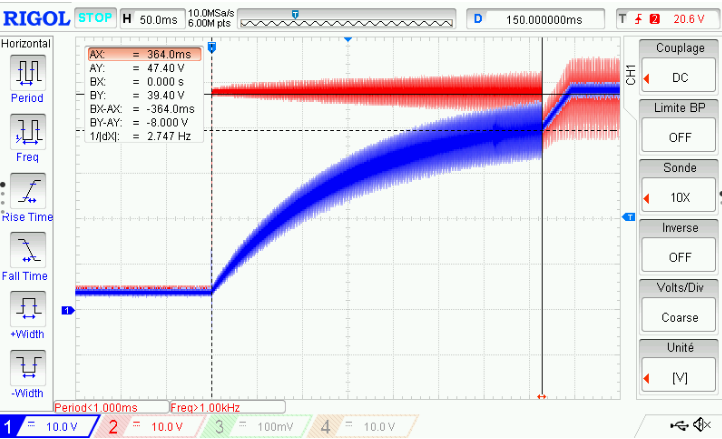
\includegraphics[width=0.75\linewidth]{assets/shared/Result_Freyche_Capa.png}
    \caption{Évolution du circuit de précharge réaliser par Thomas Freyche \cite{Freyche}}
    \label{fig:ResFreycheCapa}
\end{figure}

Lors des mesures effectuées dans le cadre de ce travail, un profil de charge identique a été relevé, comme le montre la \autoref{fig:ResCanCapa} :

\begin{figure}[H]
    \centering
    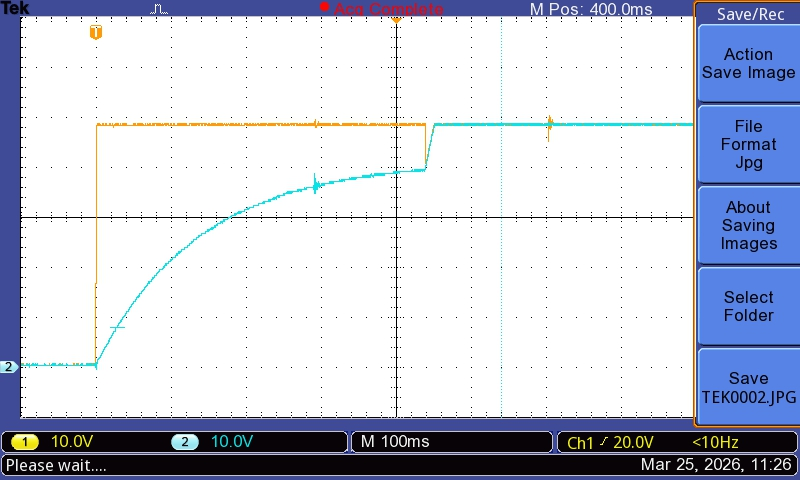
\includegraphics[width=0.75\linewidth]{assets/shared/MesureCondoCan.JPG}
    \caption{Évolution du circuit de précharge}
    \label{fig:ResCanCapa}
\end{figure}

Ces observations confirment le bon fonctionnement du circuit de précharge. Il convient toutefois de veiller à respecter scrupuleusement la durée nécessaire à la charge complète du circuit avant toute mise sous tension de l'étage de puissance.

\section{Mesure de la masse}
La masse du système a été vérifiée expérimentalement. Pour ce faire, les blocs situés à l'avant de la maquette ont été retirés afin d'extraire le module en lévitation. La masse de ce dernier a ensuite été mesurée au moyen d'une balance disponible au MakeLab et en utilisant une plaque intermédiaire afin de répartir uniformément la charge :

\begin{figure}[H]
    \centering
    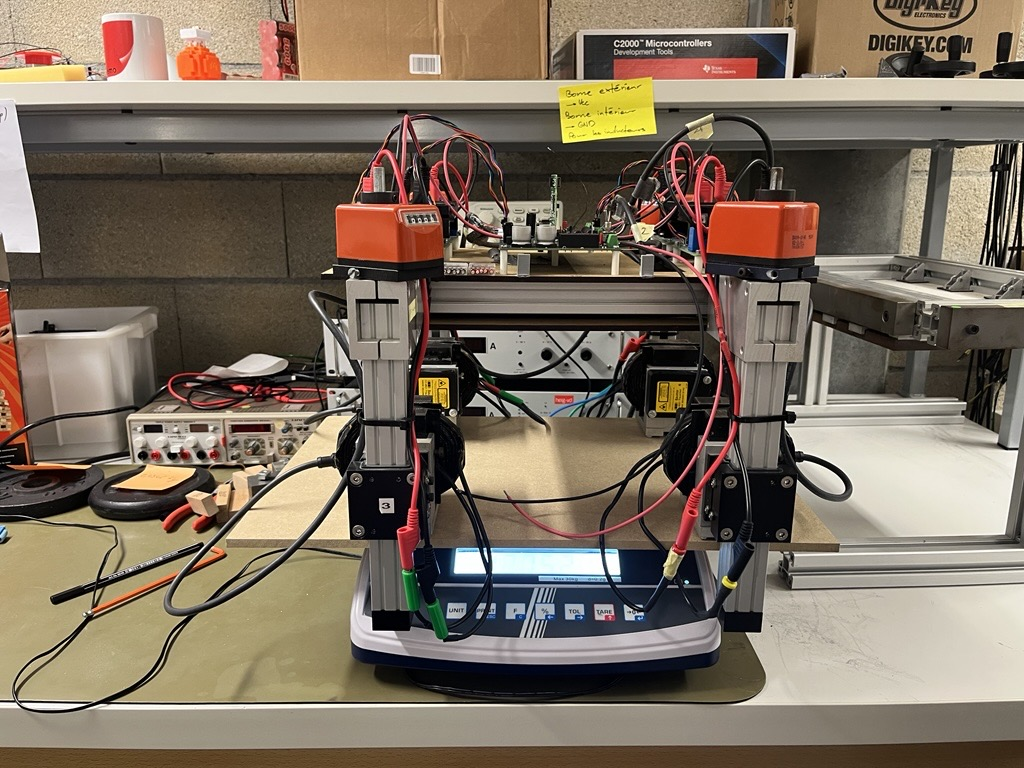
\includegraphics[width=0.75\linewidth]{assets/content/06-MesureCartePrincipale/MesureMasse.jpeg}
    \caption{Mesure de la masse totale de la partie en lévitation}
    \label{fig:mesure_masse}
\end{figure}

À la suite de cette pesée, la masse totale s'élève à 18.052~kg, contre une valeur théorique initiale de 13.6~kg.

Cette nouvelle valeur expérimentale sera par conséquent employée pour la synthèse des régulateurs ainsi que dans le code source.

\section{Mesures sur les convertisseurs DC/DC}
\label{sec:mesures_convertisseurs}
Cette section traite des relevés expérimentaux réalisés sur les convertisseurs DC/DC de la carte principale. Ces étages d'alimentation garantissent la distribution des tensions requises pour le bon fonctionnement de l'intégralité du système.

Les performances du bus principal 24~V et de l'entrée 48~V sont consignées dans le \autoref{tab:conv_24v_48v} :

\begin{table}[H]
    \centering
    \resizebox{\textwidth}{!}{%
        \begin{tabular}{|c|l|c|c|c|c|c|}
            \hline
            \multicolumn{7}{|c|}{\textbf{Convertisseur 24~V et entrée 48~V (PS1)}}                                                                                                                                                                   \\ \hline
            N°  & \multicolumn{1}{c|}{Mesure}          & Point de mesure  & \begin{tabular}[c]{@{}c@{}}Valeur théorique\\ {[}V{]}\end{tabular} & \begin{tabular}[c]{@{}c@{}}Valeur\\ mesurée {[}V{]}\end{tabular} & Erreur {[}V{]} & Erreur {[}\%]{} \\ \hline
            1.a & Entrée du 48~V                       & Bornier d'entrée & 48                                                                 & 48.05                                                            & 0.05           & 0.10            \\ \hline
            1.b & Tension après le switch de précharge & TP4              & 48                                                                 & 48.04                                                            & 0.04           & 0.08            \\ \hline
            2.a & Sortie du convertisseur 24~V         & TP6 et TP8       & 24                                                                 & 23.85                                                            & 0.15           & 0.62            \\ \hline
        \end{tabular}%
    }
    \caption{Mesures sur le convertisseur 24~V et l'entrée 48~V (PS1)}
    \label{tab:conv_24v_48v}
\end{table}

Les relevés effectués sur l'étage d'alimentation 15~V sont résumés dans le \autoref{tab:conv_15v} :

\begin{table}[H]
    \centering
    \resizebox{\textwidth}{!}{%
        \begin{tabular}{|c|l|c|c|c|c|c|}
            \hline
            \multicolumn{7}{|c|}{\textbf{Convertisseur 15~V (PS2)}}                                                                                                                                                                            \\ \hline
            N°  & \multicolumn{1}{c|}{Mesure}  & Point de mesure    & \begin{tabular}[c]{@{}c@{}}Valeur théorique\\ {[}V{]}\end{tabular} & \begin{tabular}[c]{@{}c@{}}Valeur\\ mesurée {[}V{]}\end{tabular} & Erreur {[}V{]} & Erreur {[}\%]{} \\ \hline
            1.a & Entrée du 24~V               & Côté C12 de la C13 & 24                                                                 & 23.07                                                            & 0.93           & 3.88            \\ \hline
            2.a & Sortie du convertisseur 15~V & TP1                & 15                                                                 & 14.95                                                            & 0.05           & 0.333           \\ \hline
        \end{tabular}%
    }
    \caption{Mesures sur le convertisseur 15~V (PS2)}
    \label{tab:conv_15v}
\end{table}

Le comportement du convertisseur abaisseur 5~V est présenté dans le \autoref{tab:conv_5v} :

\begin{table}[H]
    \centering
    \resizebox{\textwidth}{!}{%
        \begin{tabular}{|c|l|c|c|c|c|c|}
            \hline
            \multicolumn{7}{|c|}{\textbf{Convertisseur 5~V (IC1)}}                                                                                                                                                                              \\ \hline
            N°  & \multicolumn{1}{c|}{Mesure} & Point de mesure      & \begin{tabular}[c]{@{}c@{}}Valeur théorique\\ {[}V{]}\end{tabular} & \begin{tabular}[c]{@{}c@{}}Valeur\\ mesurée {[}V{]}\end{tabular} & Erreur {[}V{]} & Erreur {[}\%]{} \\ \hline
            1.a & Entrée du 24~V              & Pin 1 IC1            & 24                                                                 & 23.86                                                            & 0.14           & 0.583           \\ \hline
            2.a & Sortie du convertisseur 5~V & L2 côté condensateur & 5                                                                  & 4.989                                                            & 0.011          & 0.220           \\ \hline
            2.b & Après l'inducteur L2        & TP2                  & 5                                                                  & 4.987                                                            & 0.013          & 0.260           \\ \hline
        \end{tabular}%
    }
    \caption{Mesures sur le convertisseur 5~V (IC1)}
    \label{tab:conv_5v}
\end{table}

Le \autoref{tab:conv_3_3v} détaille les valeurs mesurées pour la ligne d'alimentation 3.3~V :

\begin{table}[H]
    \centering
    \resizebox{\textwidth}{!}{%
        \begin{tabular}{|c|l|c|c|c|c|c|}
            \hline
            \multicolumn{7}{|c|}{\textbf{Convertisseur 3.3~V (U6)}}                                                                                                                                                                          \\ \hline
            N°  & \multicolumn{1}{c|}{Mesure}   & Point de mesure & \begin{tabular}[c]{@{}c@{}}Valeur théorique\\ {[}V{]}\end{tabular} & \begin{tabular}[c]{@{}c@{}}Valeur\\ mesurée {[}V{]}\end{tabular} & Erreur {[}V{]} & Erreur {[}\%]{} \\ \hline
            1.a & Entrée du 5~V                 & J5 pin 2        & 5                                                                  & 4.982                                                            & 0.018          & 0.360           \\ \hline
            2.a & Sortie du convertisseur 3.3~V & TP5             & 3.3                                                                & 3.296                                                            & 0.004          & 0.121           \\ \hline
        \end{tabular}%
    }
    \caption{Mesures sur le convertisseur 3.3~V (U6)}
    \label{tab:conv_3_3v}
\end{table}

Enfin, les résultats propres à l'étage très basse tension de 0.5~V sont regroupés dans le \autoref{tab:conv_0_5v} :

\begin{table}[H]
    \centering
    \resizebox{\textwidth}{!}{%
        \begin{tabular}{|c|l|c|c|c|c|c|}
            \hline
            \multicolumn{7}{|c|}{\textbf{Convertisseur 0.5~V (U5)}}                                                                                                                                                                          \\ \hline
            N°  & \multicolumn{1}{c|}{Mesure}   & Point de mesure & \begin{tabular}[c]{@{}c@{}}Valeur théorique\\ {[}V{]}\end{tabular} & \begin{tabular}[c]{@{}c@{}}Valeur\\ mesurée {[}V{]}\end{tabular} & Erreur {[}V{]} & Erreur {[}\%]{} \\ \hline
            1.a & Entrée du 5~V                 & C18 côté U6     & 5                                                                  & 4.981                                                            & 0.019          & 0.380           \\ \hline
            2.a & Sortie du convertisseur 0.5~V & TP3             & 0.5                                                                & 0.4982                                                           & 0.0018         & 0.360           \\ \hline
        \end{tabular}%
    }
    \caption{Mesures sur le convertisseur 0.5~V (U5)}
    \label{tab:conv_0_5v}
\end{table}

\subsection{Analyse des résultats}
Les différents convertisseurs présentés ci-dessus fonctionnent de manière nominale. Les tensions fournies sont conformes aux spécifications des constructeurs, ce qui garantit une alimentation stable pour l'ensemble de la carte.

Une anomalie a néanmoins été détectée sur le convertisseur 24~V lors des essais. Une broche mal soudée provoquait l'apparition d'arcs électriques sous le circuit imprimé. Ce module devra donc faire l'objet d'une attention particulière en cas de futurs dysfonctionnements électriques. Après la reprise de la soudure, le phénomène a été éliminé.

\section{Mesures sur les capteurs de courant}
\label{sec:mesure_capteurs_courant}
Cette section présente les différents tests réalisés pour vérifier le comportement et la précision des capteurs de courant.

Dans un premier temps, le bon fonctionnement global de la chaîne d'acquisition a été vérifié, c'est-à-dire tous les composants situés entre le capteur de courant et l'entrée de l'ADC.

Ensuite, le courant mesuré avec une sonde externe a été comparé directement à la valeur lue par l'ADC. L'objectif est de vérifier la précision de la mesure embarquée et de repérer un éventuel défaut sur les capteurs en cas d'écart important entre les deux.

Pour éviter les oscillations qui peuvent apparaître quand les quatre inducteurs fonctionnent en même temps, les tests ont été faits en soulevant uniquement l'avant ou uniquement l'arrière de la maquette afin d'avoir un point de fonctionnement stable. Pour tester différentes charges, plusieurs masses ont été ajoutées sur la partie soulevée, comme montré sur la \autoref{fig:EmplacementPoids} :

\begin{figure}[H]
    \centering
    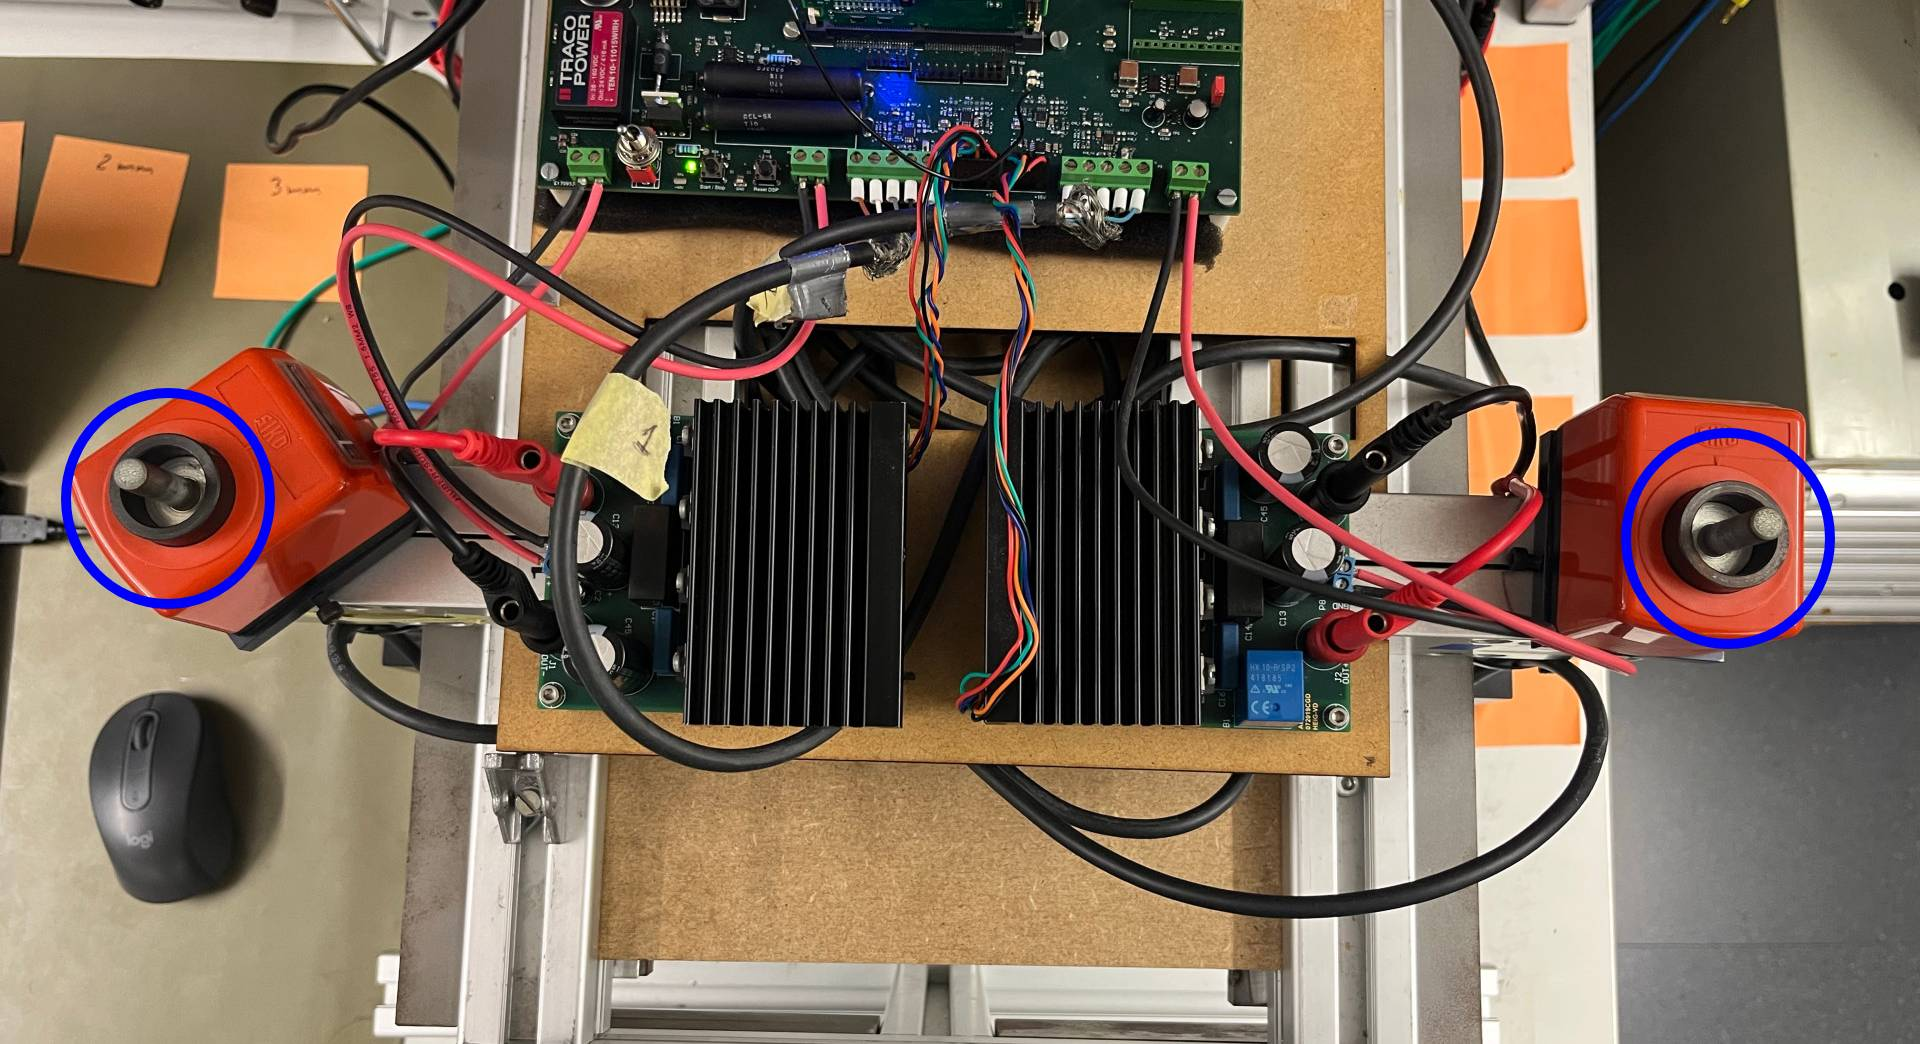
\includegraphics[width=0.75\linewidth]{assets/content/06-MesureCartePrincipale/PoidsPose.jpg}
    \caption{Emplacement des masses lors des tests}
    \label{fig:EmplacementPoids}
\end{figure}

Enfin, des comparaisons ont aussi été faites entre un calcul théorique (basé sur la masse) et les mesures réelles (sonde et ADC). Comme ces tests ont été réalisés avant de découvrir la différence de masse réelle de la maquette, leurs résultats sont moins pertinents et ont été mis dans l'\autoref{annexe:MesCour}.

\subsection{Mesure des circuits de conditionnement des capteurs de courants}

Les mesures globales des circuits de conditionnement sont présentées dans le \autoref{tab:cond_courant_1} et le \autoref{tab:cond_courant_2} :


\begin{table}[H]
    \centering
    \resizebox{\textwidth}{!}{%
        \begin{tabular}{|c|c|c|c|c|c|c|}
            \hline
            \multicolumn{7}{|c|}{\textbf{Vérification générale des conditionneurs de courant}}                                                                                                                                                                                                                                                            \\ \hline
            N°  & Mesure                                                                & \begin{tabular}[c]{@{}c@{}}Point de\\ mesure\end{tabular}   & \begin{tabular}[c]{@{}c@{}}Valeur théorique\\ {[}V{]}\end{tabular} & \begin{tabular}[c]{@{}c@{}}Valeur mesurée\\ {[}V{]}\end{tabular} & Erreur                                  & Erreur {[}\%{]} \\ \hline
            1.a & \begin{tabular}[c]{@{}c@{}}Alimentation de\\ l'AOP U1\_4\end{tabular} & U1\_4 pin 8                                                 & 5                                                                  & 4.989                                                            & 0.0110                                  & 0.2200          \\ \hline
            1.b & \begin{tabular}[c]{@{}c@{}}Alimentation de\\ l'AOP U2\_4\end{tabular} & U2\_4 pin 8                                                 & 3.3                                                                & 3.296                                                            & 0.0040                                  & 0.1212          \\ \hline
            1.c & \begin{tabular}[c]{@{}c@{}}Sortie du capteur\\ 1\end{tabular}         & \begin{tabular}[c]{@{}c@{}}R3\_4 côté\\ droite\end{tabular} & 0.625..4.375                                                       & 2.933                                                            & \multicolumn{2}{c|}{\multirow{3}{*}{-}}                   \\ \cline{1-5}
            1.d & \begin{tabular}[c]{@{}c@{}}Sortie de l'AOP\\ U1\_4\end{tabular}       & U2\_4 pin 5                                                 & 0.5..3.5                                                           & 1.173                                                            & \multicolumn{2}{c|}{}                                     \\ \cline{1-5}
            1.e & \begin{tabular}[c]{@{}c@{}}Sortie de l'AOP\\ U2\_4\end{tabular}       & TP9\_4                                                      & 0..3                                                               & 1.888                                                            & \multicolumn{2}{c|}{}                                     \\ \hline
            2.a & \begin{tabular}[c]{@{}c@{}}Alimentation de\\ l'AOP U1\_1\end{tabular} & U1\_1 pin 8                                                 & 5                                                                  & 4.984                                                            & 0.0160                                  & 0.3200          \\ \hline
            2.b & \begin{tabular}[c]{@{}c@{}}Alimentation de\\ l'AOP U2\_1\end{tabular} & U2\_1 pin 8                                                 & 3.3                                                                & 3.296                                                            & 0.0040                                  & 0.1212          \\ \hline
            2.c & \begin{tabular}[c]{@{}c@{}}Sortie du capteur\\ 2\end{tabular}         & \begin{tabular}[c]{@{}c@{}}R9\_1 côté\\ gauche\end{tabular} & 0.625..4.375                                                       & 2.872                                                            & \multicolumn{2}{c|}{\multirow{3}{*}{-}}                   \\ \cline{1-5}
            2.d & \begin{tabular}[c]{@{}c@{}}Sortie de l'AOP\\ U1\_1\end{tabular}       & U2\_1 pin 5                                                 & 0.5..3.5                                                           & 1.139                                                            & \multicolumn{2}{c|}{}                                     \\ \cline{1-5}
            2.e & \begin{tabular}[c]{@{}c@{}}Sortie de l'AOP\\ U2\_1\end{tabular}       & TP9\_1                                                      & 0..3                                                               & 1.736                                                            & \multicolumn{2}{c|}{}                                     \\ \hline
        \end{tabular}%
    }
    \caption{Vérification générale des conditionneurs de courant (Capteurs 1 et 2)}
    \label{tab:cond_courant_1}
\end{table}

\begin{table}[H]
    \centering
    \resizebox{\textwidth}{!}{%
        \begin{tabular}{|c|c|c|c|c|c|c|}
            \hline
            \multicolumn{7}{|c|}{\textbf{Vérification général des conditionneurs de courant}}                                                                                                                                                                                                                                                             \\ \hline
            N°  & Mesure                                                                & \begin{tabular}[c]{@{}c@{}}Point de\\ mesure\end{tabular}   & \begin{tabular}[c]{@{}c@{}}Valeur théorique\\ {[}V{]}\end{tabular} & \begin{tabular}[c]{@{}c@{}}Valeur mesurée\\ {[}V{]}\end{tabular} & Erreur                                  & Erreur {[}\%{]} \\ \hline
            3.a & \begin{tabular}[c]{@{}c@{}}Alimentation de\\ l'AOP U1\_3\end{tabular} & U1\_3 pin 8                                                 & 5                                                                  & 4.985                                                            & 0.0150                                  & 0.3000          \\ \hline
            3.b & \begin{tabular}[c]{@{}c@{}}Alimentation de\\ l'AOP U2\_3\end{tabular} & U2\_3 pin 8                                                 & 3.3                                                                & 3.296                                                            & 0.0040                                  & 0.1212          \\ \hline
            3.c & \begin{tabular}[c]{@{}c@{}}Sortie du capteur\\ 3\end{tabular}         & \begin{tabular}[c]{@{}c@{}}R9\_3 côté\\ droite\end{tabular} & 0.625..4.375                                                       & 2.485                                                            & \multicolumn{2}{c|}{\multirow{3}{*}{-}}                   \\ \cline{1-5}
            3.d & \begin{tabular}[c]{@{}c@{}}Sortie de l'AOP\\ U1\_3\end{tabular}       & U2\_3 pin 5                                                 & 0.5..3.5                                                           & 0.996                                                            & \multicolumn{2}{c|}{}                                     \\ \cline{1-5}
            3.e & \begin{tabular}[c]{@{}c@{}}Sortie de l'AOP\\ U2\_3\end{tabular}       & TP9\_3                                                      & 0..3                                                               & 1.532                                                            & \multicolumn{2}{c|}{}                                     \\ \hline
            4.a & \begin{tabular}[c]{@{}c@{}}Alimentation de\\ l'AOP U1\_2\end{tabular} & U1\_2 pin 8                                                 & 5                                                                  & 4.984                                                            & 0.0160                                  & 0.3200          \\ \hline
            4.b & \begin{tabular}[c]{@{}c@{}}Alimentation de\\ l'AOP U2\_2\end{tabular} & U2\_2 pin 8                                                 & 3.300                                                              & 3.296                                                            & 0.0040                                  & 0.1212          \\ \hline
            4.c & \begin{tabular}[c]{@{}c@{}}Sortie du capteur\\ 4\end{tabular}         & \begin{tabular}[c]{@{}c@{}}R9\_2 côté\\ gauche\end{tabular} & 0.625..4.375                                                       & 2.498                                                            & \multicolumn{2}{c|}{\multirow{3}{*}{-}}                   \\ \cline{1-5}
            4.d & \begin{tabular}[c]{@{}c@{}}Sortie de l'AOP\\ U1\_2\end{tabular}       & U2\_2 pin 5                                                 & 0.5..3.5                                                           & 0.999                                                            & \multicolumn{2}{c|}{}                                     \\ \cline{1-5}
            4.e & \begin{tabular}[c]{@{}c@{}}Sortie de l'AOP\\ U2\_2\end{tabular}       & TP9\_2                                                      & 0..3                                                               & 1.545                                                            & \multicolumn{2}{c|}{}                                     \\ \hline
        \end{tabular}%
    }
    \caption{Vérification générale des conditionneurs de courant (Capteurs 3 et 4)}
    \label{tab:cond_courant_2}
\end{table}

\subsection{Mesure du courant sans ajout de poids}
Une première série de mesures a été réalisée sans ajout de masse. Ces résultats sont consignés dans le \autoref{tab:sans_poids_comp} :

% --- Sans Poids - Partie 3 (Comparatif) ---
\begin{table}[H]
    \centering
    \begin{tabular}{|c|c|c|c|}
        \hline
        \multicolumn{4}{|c|}{\textbf{Sans poids}}        \\ \hline
        Inducteur & ADC {[}A{]} & Sonde {[}A{]} & Erreur \\ \hline
        1         & 6.79        & 6.08          & 0.71   \\ \hline
        2         & 6.45        & 6.16          & 0.29   \\ \hline
        3         & 6.54        & 6.40          & 0.14   \\ \hline
        4         & 6.02        & 5.84          & 0.18   \\ \hline
    \end{tabular}
    \caption{Comparatif des erreurs entre l'ADC et la sonde (Sans poids)}
    \label{tab:sans_poids_comp}
\end{table}

\subsection{Mesure du courant avec une masse de 1.25~kg}
Selon le même principe, des essais ont été effectués en ajoutant une masse d'environ 1.25 kg. Les mesures correspondantes sont présentées dans le \autoref{tab:poids_1_25_comp} :

% --- Poids 1.25 kg - Partie 3 (Comparatif) ---
\begin{table}[H]
    \centering
    \begin{tabular}{|c|c|c|c|}
        \hline
        \multicolumn{4}{|c|}{\textbf{Poids de 1.25 kg}}  \\ \hline
        Inducteur & ADC {[}A{]} & Sonde {[}A{]} & Erreur \\ \hline
        1         & 8.0         & 7.6           & 0.38   \\ \hline
        2         & 7.3         & 7.2           & 0.060  \\ \hline
        3         & 7.5         & 7.4           & 0.065  \\ \hline
        4         & 7.1         & 7.2           & 0.10   \\ \hline
    \end{tabular}
    \caption{Comparatif des erreurs entre l'ADC et la sonde (Poids de 1.25 kg)}
    \label{tab:poids_1_25_comp}
\end{table}

\subsection{Mesure du courant avec une masse de 2.5~kg}
Enfin, une charge d'environ 2.5~kg a été ajoutée pour clore les essais. Les résultats de ces mesures sont détaillés dans le \autoref{tab:poids_2_5_comp} :

% --- Poids 2.5 kg - Partie 3 (Comparatif) ---
\begin{table}[H]
    \centering
    \begin{tabular}{|c|c|c|c|}
        \hline
        \multicolumn{4}{|c|}{\textbf{Poids de 2.5 kg}}   \\ \hline
        Inducteur & ADC {[}A{]} & Sonde {[}A{]} & Erreur \\ \hline
        1         & 8.9         & 8.2           & 0.73   \\ \hline
        2         & 8.3         & 8.2           & 0.093  \\ \hline
        3         & 8.1         & 8.2           & 0.15   \\ \hline
        4         & 8.8         & 8.8           & 0.022  \\ \hline
    \end{tabular}
    \caption{Comparatif des erreurs entre l'ADC et la sonde (Poids de 2.5 kg)}
    \label{tab:poids_2_5_comp}
\end{table}

\subsection{Analyse des résultats}
La comparaison des deux méthodes de mesure, illustrée du \autoref{tab:sans_poids_comp} au \autoref{tab:poids_2_5_comp}, met en évidence une forte corrélation entre les résultats. Cela démontre la fiabilité de la chaîne d'acquisition des données et confirme l'exactitude de la correspondance entre le courant circulant réellement dans l'inducteur et la valeur numérique lue par le capteur.

Le fonctionnement du capteur de courant est par conséquent validé.

\section{Mesure des capteurs de position}
Cette section traite des mesures réalisées sur les capteurs de position. L'étalonnage précédent a été réalisé de la manière suivante :

\begin{minted}{c}
// 3722.7 / 3500 = 1.06, valeur 12 bit pour 3mm / valeur mesuree ADC (2.8mm) = ecart
Position1 = (float)(ADC_pos_1) * CONV_POS2 * POS_CORRECTION_1;
// 3722.7 / 3480 = 1.07, valeur 12 bit pour 3mm / valeur mesuree ADC (2.8mm) = ecart
Position2 = (float)(ADC_pos_2) * CONV_POS2 * POS_CORRECTION_2;
Position3 = (float)(ADC_pos_3) * CONV_POS2 * POS_CORRECTION_1;
Position4 = (float)(ADC_pos_4) * CONV_POS2 * POS_CORRECTION_2;
\end{minted}

L'approche consistant à multiplier un gain similaire pour les inducteurs 3 et 4 laissant à désirer, de nombreuses séries d'essais ont été effectuées afin d'améliorer l'étalonnage. Seule la dernière approche a été conservée afin d'alléger le contenu de ce document ; les autres sont disponibles dans l'\autoref{annexe:MesPos}.

Il a également été décidé de réaliser une nouvelle calibration teach-in des capteurs de position. Cela s'explique par le fait que la calibration précédente avait été réalisée en levant uniquement l'arrière ou uniquement l'avant. Cette démarche visait aussi à éliminer un angle pouvant se créer entre les capteurs avant et arrière, comme indiqué sur la \autoref{fig:MaqCote} :

\begin{figure}[H]
    \centering
    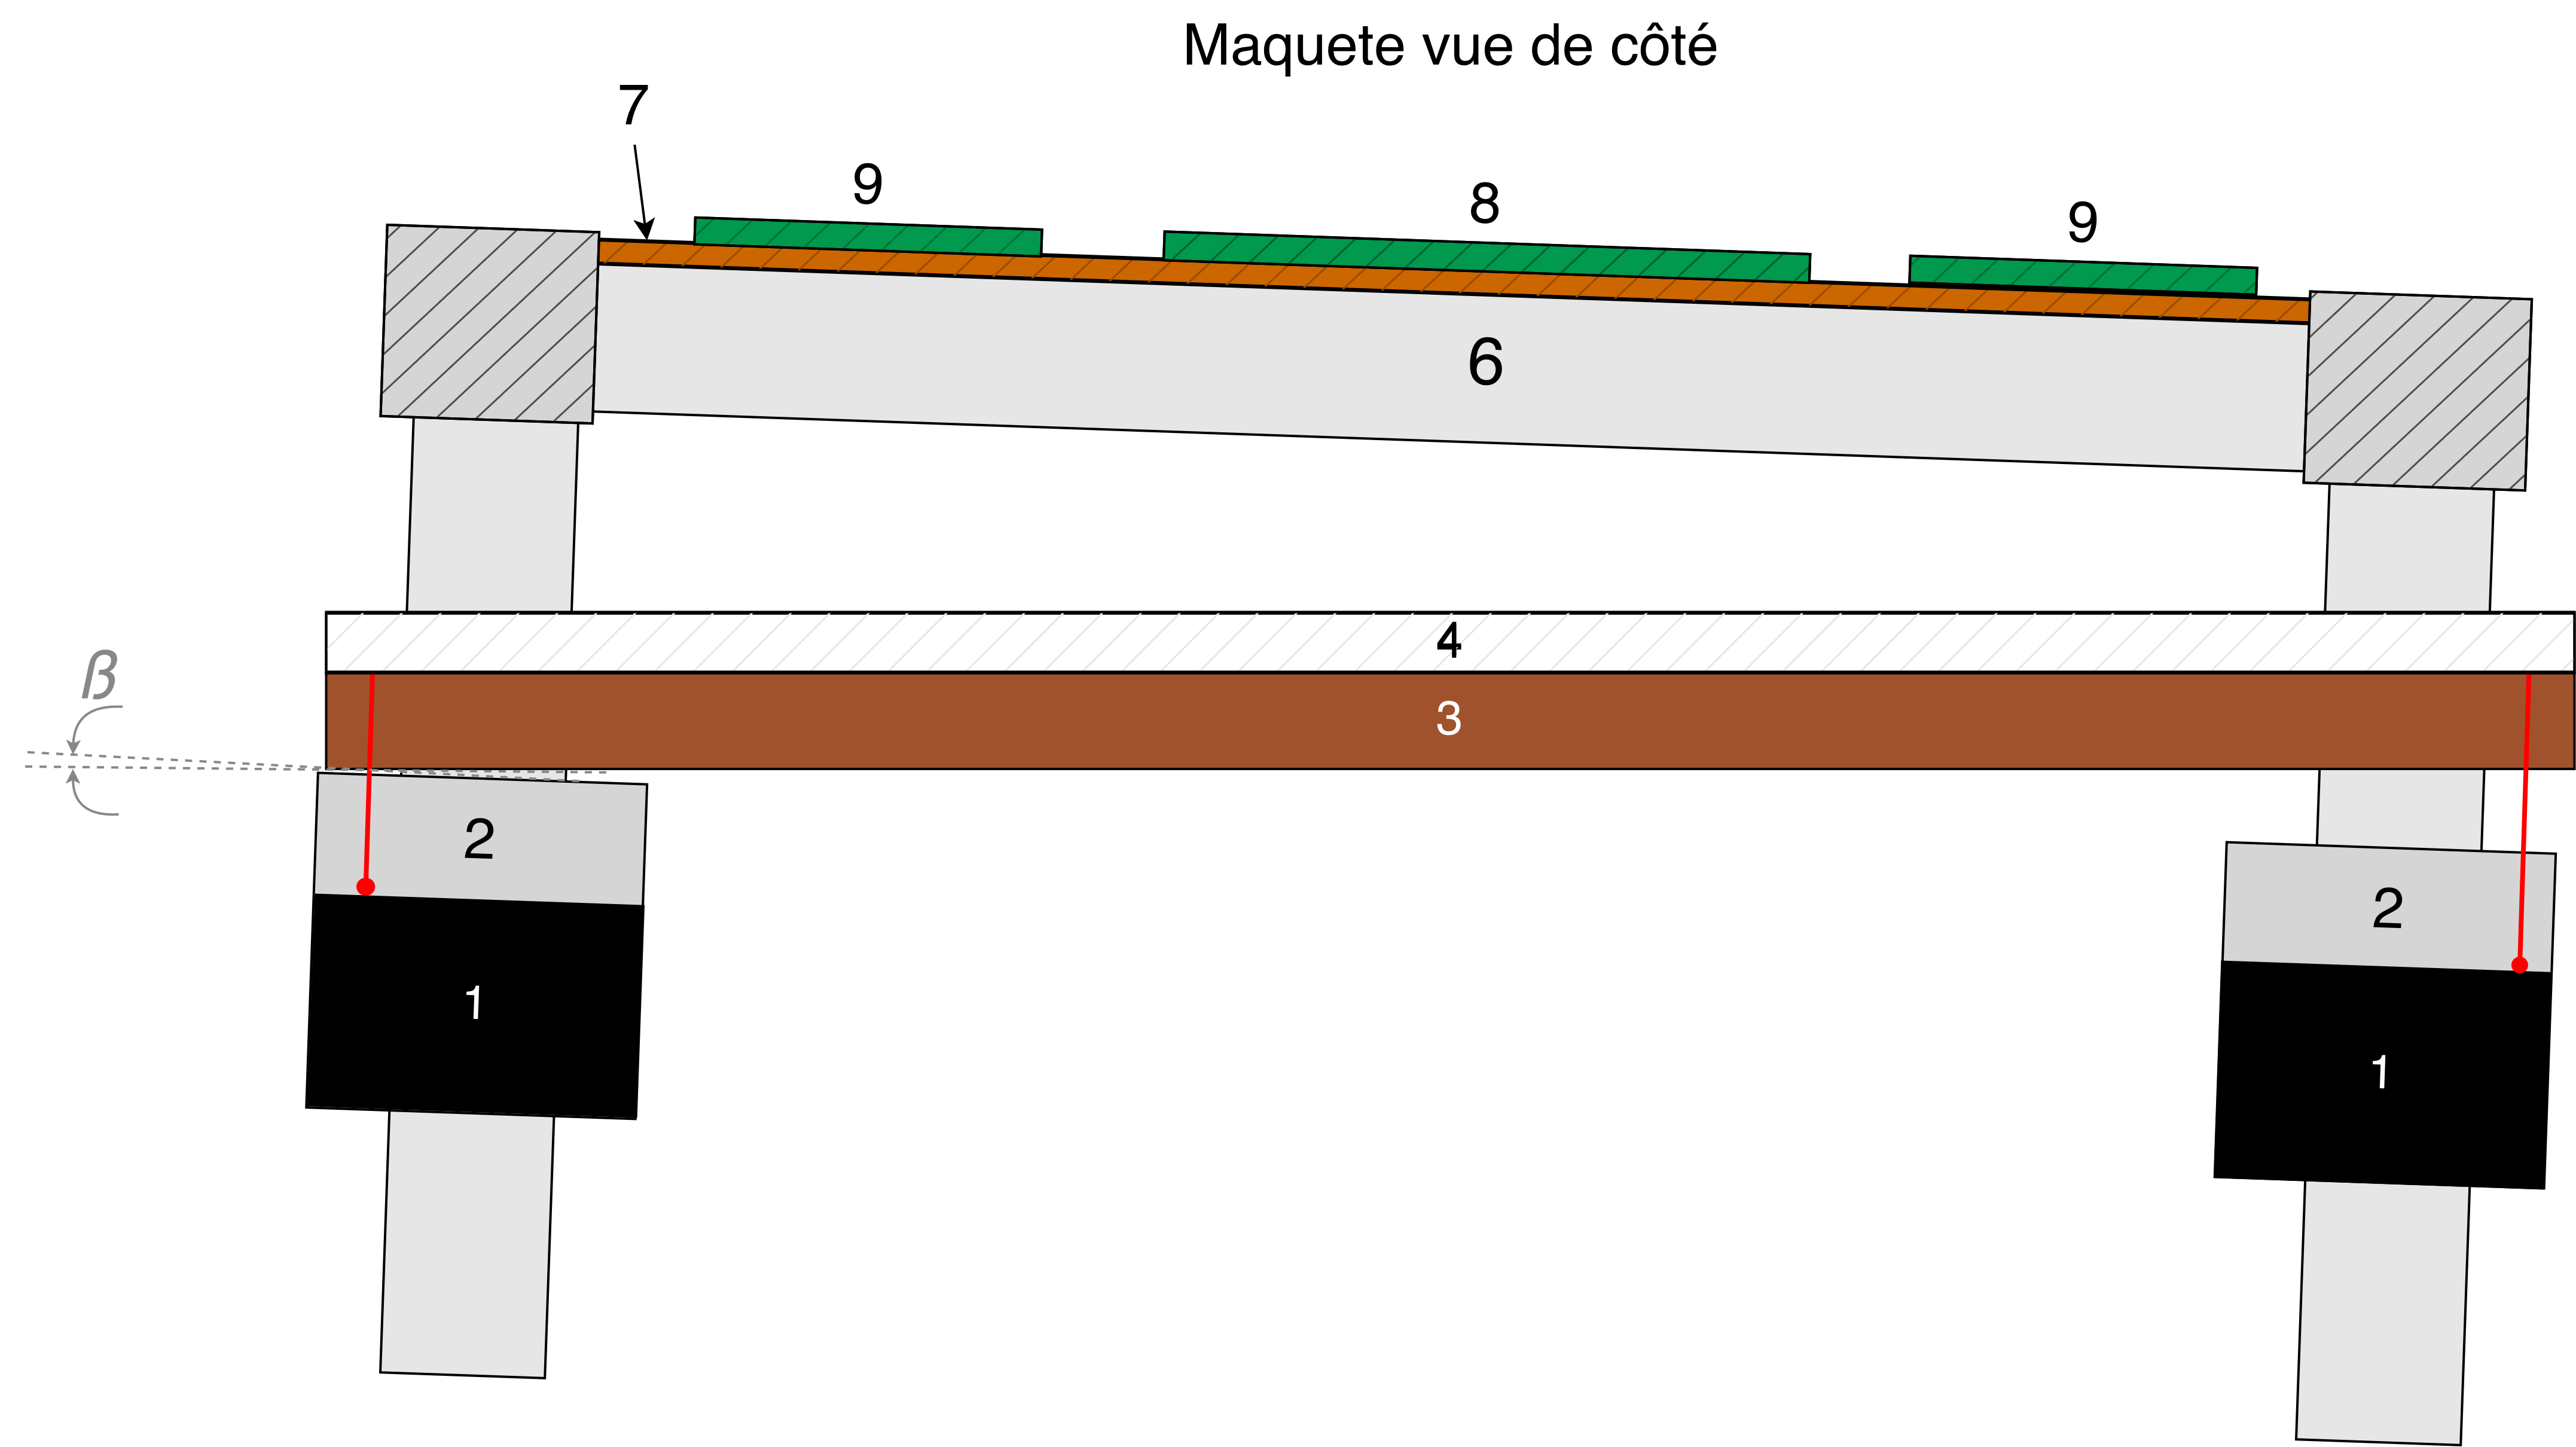
\includegraphics[width=1\linewidth]{assets/shared/MaquetteCote.png}
    \caption{Calibration en levant uniquement un côté(Avant ou arrière)}
    \label{fig:MaqCote}
\end{figure}

Avec 7 la plaque en bois, 8 la carte principale et 9 les cartes de puissances.

La calibration a été réalisée à une même hauteur en suivant les étapes décrites dans l'\autoref{sec:CalibrationCaptPosManuel}.

Les mesures ont été réalisées à l'aide de cales de différentes épaisseurs (1~mm, 1.5~mm, 2~mm et 3~mm). Ces éléments permettaient de surélever la partie mobile et, ainsi, de réduire l'entrefer des bobines. Dans les relevés, un entrefer de 3~mm correspond à la position de repos théorique du chariot. Lorsqu'une cale de 2.5~mm est mentionnée, cela correspond à la superposition d'une cale de 1~mm et d'une cale de 1.5~mm. La correspondance cale et entrefer est la suivante :

\begin{table}[H]
    \centering
    \begin{tabular}{cc}
        \toprule
        \textbf{Cales [mm]} & \textbf{Entrefer [mm]} \\
        \midrule
        0                   & 3                      \\
        1                   & 2                      \\
        1.5                 & 1.5                    \\
        2                   & 1                      \\
        2.5                 & 0.5                    \\
        3                   & 0                      \\
        \bottomrule
    \end{tabular}
    \caption{Relation entre les calles et l'entrefer}
    \label{tab:calles_entrefer}
\end{table}

Les mesures sont réalisé en affichant la valeur de l'adc filtré sur l'interface web.

\subsection{Mesure des circuits de conditionnement}
Dans un premier temps, une vérification globale des circuits de conditionnement a été effectuée, de manière analogue à la procédure suivie pour les capteurs de courant. Les résultats sont présentés dans le \autoref{tab:cond_position} :

\begin{table}[H]
    \centering
    \resizebox{\textwidth}{!}{%
        \begin{tabular}{|c|c|c|c|c|c|c|}
            \hline
            \multicolumn{7}{|c|}{\textbf{Vérification générale des conditionneurs de position}}                                                                                                                                                                                                                                                           \\ \hline
            N°  & Mesure                                                                & \begin{tabular}[c]{@{}c@{}}Point de\\ mesure\end{tabular}   & \begin{tabular}[c]{@{}c@{}}Valeur\\ théorique {[}V{]}\end{tabular} & \begin{tabular}[c]{@{}c@{}}Valeur\\ mesurée {[}V{]}\end{tabular} & Erreur                                  & Erreur {[}\%{]} \\ \hline
            1.a & \begin{tabular}[c]{@{}c@{}}Alimentation de\\ l'AOP U3\_4\end{tabular} & U3\_4 pin 8                                                 & 3.3                                                                & 3.30                                                             & 4E-03                                   & 0.12            \\ \hline
            1.c & Sortie du capteur 1                                                   & \begin{tabular}[c]{@{}c@{}}Connector 1\\ pin 2\end{tabular} & 0..10                                                              & 9.56                                                             & \multicolumn{2}{c|}{\multirow{2}{*}{-}}                   \\ \cline{1-5}
            1.d & Sortie de l'AOP U1\_4                                                 & TP12\_4                                                     & 0..3                                                               & 2.85                                                             & \multicolumn{2}{c|}{}                                     \\ \hline
            2.a & \begin{tabular}[c]{@{}c@{}}Alimentation de\\ l'AOP U3\_1\end{tabular} & U3\_1 pin 8                                                 & 3.3                                                                & 3.30                                                             & 4E-03                                   & 0.12            \\ \hline
            2.c & Sortie du capteur 2                                                   & \begin{tabular}[c]{@{}c@{}}Connector 2\\ pin 2\end{tabular} & 0..10                                                              & 9.74                                                             & \multicolumn{2}{c|}{\multirow{2}{*}{-}}                   \\ \cline{1-5}
            2.d & Sortie de l'AOP U3\_1                                                 & TP12\_1                                                     & 0..3                                                               & 2.91                                                             & \multicolumn{2}{c|}{}                                     \\ \hline
            3.a & \begin{tabular}[c]{@{}c@{}}Alimentation de\\ l'AOP U3\_3\end{tabular} & U3\_3 pin 8                                                 & 3.3                                                                & 3.30                                                             & 4E-03                                   & 0.12            \\ \hline
            3.c & Sortie du capteur 3                                                   & \begin{tabular}[c]{@{}c@{}}Connector 3\\ pin 2\end{tabular} & 0..10                                                              & 9.92                                                             & \multicolumn{2}{c|}{\multirow{2}{*}{-}}                   \\ \cline{1-5}
            3.d & Sortie de l'AOP U1\_3                                                 & U3\_3 pin 5                                                 & 0..3                                                               & 2.96                                                             & \multicolumn{2}{c|}{}                                     \\ \hline
            4.a & \begin{tabular}[c]{@{}c@{}}Alimentation de\\ l'AOP U3\_2\end{tabular} & U3\_2 pin 8                                                 & 3.3                                                                & 3.30                                                             & 4E-03                                   & 0.12            \\ \hline
            4.c & Sortie du capteur 4                                                   & \begin{tabular}[c]{@{}c@{}}Connector 4\\ pin 2\end{tabular} & 0..10                                                              & 10.0                                                             & \multicolumn{2}{c|}{\multirow{2}{*}{-}}                   \\ \cline{1-5}
            4.d & Sortie de l'AOP U3\_2                                                 & TP12\_2                                                     & 0..3                                                               & 2.99                                                             & \multicolumn{2}{c|}{}                                     \\ \hline
        \end{tabular}%
    }
    \caption{Vérification générale des conditionneurs de position}
    \label{tab:cond_position}
\end{table}

\subsection{Mesure d'étalonnage des valeurs d'ADC}
Face à l'absence de résultats concluants, l'application d'une correction directe sur la valeur numérique de l'ADC a été testée. Lors des travaux antérieurs, la valeur brute de l'ADC était convertie par une constante \texttt{CONV\_POS2} (Voir \autoref{subsec:Conditionneur}).

Afin d'obtenir une mesure de position plus précise et spécifique à chaque inducteur, une nouvelle fonction de transfert a été développée pour convertir directement le signal brut de l'ADC en une grandeur physique exprimée en mètre.

\begin{table}[H]
    \centering
    \resizebox{\textwidth}{!}{%
        \begin{tabular}{|c|c|c|c|c|c|c|c|c|}
            \hline
            \multicolumn{9}{|c|}{\textbf{Mesure des positions brutes de l'ADC pour l'inducteur 1}}                                                                                                                                                                                                                                         \\ \hline
            Ligne              & Entrefer {[}m{]} & Théorique & \begin{tabular}[c]{@{}c@{}}Mesure\\ au centre\end{tabular} & \begin{tabular}[c]{@{}c@{}}Mesure\\ à gauche\end{tabular} & \begin{tabular}[c]{@{}c@{}}Mesure\\ à droite\end{tabular} & Moyenne & Erreur & \begin{tabular}[c]{@{}c@{}}Erreur\\ relative {[}\%{]}\end{tabular} \\ \hline
            \multirow{6}{*}{1} & 3.00E-03         & 3723      & 3492                                                       & 3490                                                      & 3492                                                      & 3492    & 231    & 6.20                                                               \\ \cline{2-9}
                               & 2.50E-03         & 3103      & 2599                                                       & 2699                                                      & 2568                                                      & 2622    & 481    & 15.50                                                              \\ \cline{2-9}
                               & 2.00E-03         & 2482      & 2096                                                       & 2171                                                      & 2040                                                      & 2103    & 379    & 15.3                                                               \\ \cline{2-9}
                               & 1.50E-03         & 1862      & 1467                                                       & 1552                                                      & 1379                                                      & 1466    & 396    & 21.3                                                               \\ \cline{2-9}
                               & 1.00E-03         & 1241      & 747                                                        & 826                                                       & 703                                                       & 759     & 482    & 38.8                                                               \\ \cline{2-9}
                               & 0.00E+00         & 0         & 432                                                        & 527                                                       & 393                                                       & 451     & 451    & -                                                                  \\ \hline
            \multirow{6}{*}{2} & 3.00E-03         & 3723      & 3492                                                       & 3488                                                      & 3493                                                      & 3491    & 232    & 6.23                                                               \\ \cline{2-9}
                               & 2.50E-03         & 3103      & 2484                                                       & 2549                                                      & 2451                                                      & 2495    & 608    & 19.594                                                             \\ \cline{2-9}
                               & 2.00E-03         & 2482      & 2025                                                       & 2074                                                      & 1976                                                      & 2025    & 457    & 18.41                                                              \\ \cline{2-9}
                               & 1.50E-03         & 1862      & 1350                                                       & 1429                                                      & 1321                                                      & 1367    & 495    & 26.6                                                               \\ \cline{2-9}
                               & 1.00E-03         & 1241      & 699                                                        & 743                                                       & 650                                                       & 698     & 543    & 43.8                                                               \\ \cline{2-9}
                               & 0.00E+00         & 0         & 321                                                        & 401                                                       & 261                                                       & 328     & 328    & -                                                                  \\ \hline
            \multirow{6}{*}{3} & 3.00E-03         & 3723      & 3491                                                       & 3488                                                      & 3488                                                      & 3489    & 234    & 6.29                                                               \\ \cline{2-9}
                               & 2.50E-03         & 3103      & 2423                                                       & 2315                                                      & 2419                                                      & 2386    & 717    & 23.11                                                              \\ \cline{2-9}
                               & 2.00E-03         & 2482      & 1902                                                       & 1903                                                      & 1874                                                      & 1893    & 589    & 23.73                                                              \\ \cline{2-9}
                               & 1.50E-03         & 1862      & 1199                                                       & 1216                                                      & 1187                                                      & 1201    & 661    & 35.50                                                              \\ \cline{2-9}
                               & 1.00E-03         & 1241      & 476                                                        & 522                                                       & 465                                                       & 488     & 753    & 60.7                                                               \\ \cline{2-9}
                               & 0.00E+00         & 0         & 230                                                        & 221                                                       & 162                                                       & 205     & 205    & -                                                                  \\ \hline
            \multirow{6}{*}{4} & 3.00E-03         & 3723      & 3486                                                       & 3483                                                      & 3492                                                      & 3487    & 236    & 6.34                                                               \\ \cline{2-9}
                               & 2.50E-03         & 3103      & 2452                                                       & 2417                                                      & 2410                                                      & 2427    & 676    & 21.79                                                              \\ \cline{2-9}
                               & 2.00E-03         & 2482      & 1903                                                       & 1912                                                      & 1851                                                      & 1889    & 593    & 23.89                                                              \\ \cline{2-9}
                               & 1.50E-03         & 1862      & 1264                                                       & 1292                                                      & 1193                                                      & 1250    & 612    & 32.868                                                             \\ \cline{2-9}
                               & 1.00E-03         & 1241      & 494                                                        & 507                                                       & 453                                                       & 485     & 756    & 60.9                                                               \\ \cline{2-9}
                               & 0.00E+00         & 0         & 148                                                        & 186                                                       & 142                                                       & 159     & 159    & -                                                                  \\ \hline
            \multirow{6}{*}{5} & 3.00E-03         & 3723      & 3486                                                       & 3485                                                      & 3489                                                      & 3487    & 236    & 6.34                                                               \\ \cline{2-9}
                               & 2.50E-03         & 3103      & 2496                                                       & 2527                                                      & 2515                                                      & 2513    & 590    & 19.01                                                              \\ \cline{2-9}
                               & 2.00E-03         & 2482      & 1969                                                       & 1997                                                      & 1881                                                      & 1949    & 533    & 21.47                                                              \\ \cline{2-9}
                               & 1.50E-03         & 1862      & 1300                                                       & 1367                                                      & 1196                                                      & 1288    & 574    & 30.83                                                              \\ \cline{2-9}
                               & 1.00E-03         & 1241      & 518                                                        & 599                                                       & 572                                                       & 563     & 678    & 54.63                                                              \\ \cline{2-9}
                               & 0.00E+00         & 0         & 277                                                        & 341                                                       & 243                                                       & 287     & 287    & -                                                                  \\ \hline
        \end{tabular}%
    }
    \caption{Mesure des positions brutes de l'ADC pour l'inducteur 1}
    \label{tab:adc_brut_inducteur1}
\end{table}

\begin{table}[H]
    \centering
    \resizebox{\textwidth}{!}{%
        \begin{tabular}{|c|c|c|c|c|c|c|c|c|}
            \hline
            \multicolumn{9}{|c|}{\textbf{Mesure des positions brutes de l'ADC pour l'inducteur 2}}                                                                                                                                                                                                                                         \\ \hline
            Ligne              & Entrefer {[}m{]} & Théorique & \begin{tabular}[c]{@{}c@{}}Mesure\\ au centre\end{tabular} & \begin{tabular}[c]{@{}c@{}}Mesure\\ à gauche\end{tabular} & \begin{tabular}[c]{@{}c@{}}Mesure\\ à droite\end{tabular} & Moyenne & Erreur & \begin{tabular}[c]{@{}c@{}}Erreur\\ relative {[}\%{]}\end{tabular} \\ \hline
            \multirow{6}{*}{1} & 3.00E-03         & 3723      & 3518                                                       & 3518                                                      & 3518                                                      & 3518    & 205    & 5.51                                                               \\ \cline{2-9}
                               & 2.50E-03         & 3103      & 2441                                                       & 2388                                                      & 2521                                                      & 2450    & 653    & 21.04                                                              \\ \cline{2-9}
                               & 2.00E-03         & 2482      & 1907                                                       & 1849                                                      & 1931                                                      & 1896    & 586    & 23.61                                                              \\ \cline{2-9}
                               & 1.50E-03         & 1862      & 1291                                                       & 1261                                                      & 1340                                                      & 1298    & 564    & 30.29                                                              \\ \cline{2-9}
                               & 1.00E-03         & 1241      & 609                                                        & 550                                                       & 681                                                       & 614     & 627    & 50.52                                                              \\ \cline{2-9}
                               & 0.00E+00         & 0         & 317                                                        & 247                                                       & 354                                                       & 306     & 306    & -                                                                  \\ \hline
            \multirow{6}{*}{2} & 3.00E-03         & 3723      & 3518                                                       & 3518                                                      & 3518                                                      & 3518    & 205    & 5.51                                                               \\ \cline{2-9}
                               & 2.50E-03         & 3103      & 2358                                                       & 2281                                                      & 2390                                                      & 2343    & 760    & 24.49                                                              \\ \cline{2-9}
                               & 2.00E-03         & 2482      & 1843                                                       & 1778                                                      & 1888                                                      & 1837    & 645    & 25.99                                                              \\ \cline{2-9}
                               & 1.50E-03         & 1862      & 1248                                                       & 1196                                                      & 1281                                                      & 1242    & 620    & 33.2975                                                            \\ \cline{2-9}
                               & 1.00E-03         & 1241      & 579                                                        & 496                                                       & 643                                                       & 573     & 668    & 53.83                                                              \\ \cline{2-9}
                               & 0.00E+00         & 0         & 204                                                        & 104                                                       & 233                                                       & 181     & 181    & -                                                                  \\ \hline
            \multirow{6}{*}{3} & 3.00E-03         & 3723      & 3518                                                       & 3518                                                      & 3518                                                      & 3518    & 205    & 5.51                                                               \\ \cline{2-9}
                               & 2.50E-03         & 3103      & 2443                                                       & 2316                                                      & 2499                                                      & 2420    & 683    & 22.01                                                              \\ \cline{2-9}
                               & 2.00E-03         & 2482      & 1871                                                       & 1788                                                      & 1913                                                      & 1858    & 624    & 25.141                                                             \\ \cline{2-9}
                               & 1.50E-03         & 1862      & 1231                                                       & 1147                                                      & 1277                                                      & 1219    & 643    & 34.53                                                              \\ \cline{2-9}
                               & 1.00E-03         & 1241      & 503                                                        & 463                                                       & 586                                                       & 518     & 723    & 58.3                                                               \\ \cline{2-9}
                               & 0.00E+00         & 0         & 148                                                        & 59                                                        & 239                                                       & 149     & 149    & -                                                                  \\ \hline
            \multirow{6}{*}{4} & 3.00E-03         & 3723      & 3518                                                       & 3518                                                      & 3518                                                      & 3518    & 205    & 5.51                                                               \\ \cline{2-9}
                               & 2.50E-03         & 3103      & 2486                                                       & 2428                                                      & 2635                                                      & 2517    & 586    & 18.88                                                              \\ \cline{2-9}
                               & 2.00E-03         & 2482      & 1997                                                       & 1945                                                      & 2078                                                      & 2007    & 475    & 19.14                                                              \\ \cline{2-9}
                               & 1.50E-03         & 1862      & 1361                                                       & 1294                                                      & 1432                                                      & 1363    & 499    & 26.80                                                              \\ \cline{2-9}
                               & 1.00E-03         & 1241      & 630                                                        & 568                                                       & 734                                                       & 644     & 597    & 48.11                                                              \\ \cline{2-9}
                               & 0.00E+00         & 0         & 149                                                        & 62                                                        & 230                                                       & 147     & 147    & -                                                                  \\ \hline
            \multirow{6}{*}{5} & 3.00E-03         & 3723      & 3518                                                       & 3518                                                      & 3518                                                      & 3518    & 205    & 5.51                                                               \\ \cline{2-9}
                               & 2.50E-03         & 3103      & 2478                                                       & 2428                                                      & 2422                                                      & 2443    & 660    & 21.27                                                              \\ \cline{2-9}
                               & 2.00E-03         & 2482      & 1938                                                       & 1890                                                      & 2043                                                      & 1957    & 525    & 21.15                                                              \\ \cline{2-9}
                               & 1.50E-03         & 1862      & 1375                                                       & 1293                                                      & 1420                                                      & 1363    & 499    & 26.80                                                              \\ \cline{2-9}
                               & 1.00E-03         & 1241      & 620                                                        & 586                                                       & 541                                                       & 583     & 658    & 53.02                                                              \\ \cline{2-9}
                               & 0.00E+00         & 0         & 269                                                        & 228                                                       & 284                                                       & 261     & 261    & -                                                                  \\ \hline
        \end{tabular}%
    }
    \caption{Mesure des positions brutes de l'ADC pour l'inducteur 2}
    \label{tab:adc_brut_inducteur2}
\end{table}

\begin{table}[H]
    \centering
    \resizebox{\textwidth}{!}{%
        \begin{tabular}{|c|c|c|c|c|c|c|c|c|}
            \hline
            \multicolumn{9}{|c|}{\textbf{Mesure des positions brutes de l'ADC pour l'inducteur 3}}                                                                                                                                                                                                                                         \\ \hline
            Ligne              & Entrefer {[}m{]} & Théorique & \begin{tabular}[c]{@{}c@{}}Mesure\\ au centre\end{tabular} & \begin{tabular}[c]{@{}c@{}}Mesure\\ à gauche\end{tabular} & \begin{tabular}[c]{@{}c@{}}Mesure\\ à droite\end{tabular} & Moyenne & Erreur & \begin{tabular}[c]{@{}c@{}}Erreur\\ relative {[}\%{]}\end{tabular} \\ \hline
            \multirow{6}{*}{1} & 3.00E-03         & 3723      & 3486                                                       & 3486                                                      & 3486                                                      & 3486    & 237    & 6.37                                                               \\ \cline{2-9}
                               & 2.50E-03         & 3103      & 2385                                                       & 2475                                                      & 2333                                                      & 2398    & 705    & 22.72                                                              \\ \cline{2-9}
                               & 2.00E-03         & 2482      & 1811                                                       & 1914                                                      & 1779                                                      & 1835    & 647    & 26.07                                                              \\ \cline{2-9}
                               & 1.50E-03         & 1862      & 1206                                                       & 1226                                                      & 1127                                                      & 1187    & 675    & 36.25                                                              \\ \cline{2-9}
                               & 1.00E-03         & 1241      & 506                                                        & 502                                                       & 467                                                       & 492     & 749    & 60.4                                                               \\ \cline{2-9}
                               & 0.00E+00         & 0         & 104                                                        & 40                                                        & 106                                                       & 84      & 84     & -                                                                  \\ \hline
            \multirow{6}{*}{2} & 3.00E-03         & 3723      & 3487                                                       & 3487                                                      & 3487                                                      & 3487    & 236    & 6.34                                                               \\ \cline{2-9}
                               & 2.50E-03         & 3103      & 2230                                                       & 2265                                                      & 2208                                                      & 2235    & 868    & 27.97                                                              \\ \cline{2-9}
                               & 2.00E-03         & 2482      & 1651                                                       & 1706                                                      & 1615                                                      & 1658    & 824    & 33.2                                                               \\ \cline{2-9}
                               & 1.50E-03         & 1862      & 1053                                                       & 1071                                                      & 990                                                       & 1038    & 824    & 44.3                                                               \\ \cline{2-9}
                               & 1.00E-03         & 1241      & 237                                                        & 274                                                       & 198                                                       & 237     & 1004   & 80.9                                                               \\ \cline{2-9}
                               & 0.00E+00         & 0         & 27                                                         & 20                                                        & 29                                                        & 26      & 26     & -                                                                  \\ \hline
            \multirow{6}{*}{3} & 3.00E-03         & 3723      & 3486                                                       & 3487                                                      & 3487                                                      & 3487    & 236    & 6.34                                                               \\ \cline{2-9}
                               & 2.50E-03         & 3103      & 2111                                                       & 2153                                                      & 2117                                                      & 2127    & 976    & 31.45                                                              \\ \cline{2-9}
                               & 2.00E-03         & 2482      & 1657                                                       & 1666                                                      & 1600                                                      & 1641    & 841    & 33.88                                                              \\ \cline{2-9}
                               & 1.50E-03         & 1862      & 972                                                        & 962                                                       & 982                                                       & 972     & 890    & 47.80                                                              \\ \cline{2-9}
                               & 1.00E-03         & 1241      & 264                                                        & 299                                                       & 250                                                       & 271     & 970    & 78.2                                                               \\ \cline{2-9}
                               & 0.00E+00         & 0         & 52                                                         & 18                                                        & 30                                                        & 34      & 34     & -                                                                  \\ \hline
            \multirow{6}{*}{4} & 3.00E-03         & 3723      & 3487                                                       & 3487                                                      & 3474                                                      & 3483    & 240    & 6.45                                                               \\ \cline{2-9}
                               & 2.50E-03         & 3103      & 2289                                                       & 2359                                                      & 2195                                                      & 2281    & 822    & 26.49                                                              \\ \cline{2-9}
                               & 2.00E-03         & 2482      & 1736                                                       & 1811                                                      & 1649                                                      & 1732    & 750    & 30.22                                                              \\ \cline{2-9}
                               & 1.50E-03         & 1862      & 1123                                                       & 1182                                                      & 977                                                       & 1094    & 768    & 41.2                                                               \\ \cline{2-9}
                               & 1.00E-03         & 1241      & 362                                                        & 431                                                       & 300                                                       & 365     & 876    & 70.6                                                               \\ \cline{2-9}
                               & 0.00E+00         & 0         & 142                                                        & 126                                                       & 98                                                        & 122     & 122    & -                                                                  \\ \hline
            \multirow{6}{*}{5} & 3.00E-03         & 3723      & 3487                                                       & 3487                                                      & 3487                                                      & 3487    & 236    & 6.34                                                               \\ \cline{2-9}
                               & 2.50E-03         & 3103      & 2340                                                       & 2425                                                      & 2407                                                      & 2391    & 712    & 22.95                                                              \\ \cline{2-9}
                               & 2.00E-03         & 2482      & 1855                                                       & 1919                                                      & 1780                                                      & 1852    & 630    & 25.383                                                             \\ \cline{2-9}
                               & 1.50E-03         & 1862      & 1173                                                       & 1261                                                      & 1120                                                      & 1185    & 677    & 36.36                                                              \\ \cline{2-9}
                               & 1.00E-03         & 1241      & 487                                                        & 587                                                       & 545                                                       & 540     & 701    & 56.5                                                               \\ \cline{2-9}
                               & 0.00E+00         & 0         & 281                                                        & 266                                                       & 225                                                       & 258     & 258    & -                                                                  \\ \hline
        \end{tabular}%
    }
    \caption{Mesure des positions brutes de l'ADC pour l'inducteur 3}
    \label{tab:adc_brut_inducteur3}
\end{table}

\begin{table}[H]
    \centering
    \resizebox{\textwidth}{!}{%
        \begin{tabular}{|c|c|c|c|c|c|c|c|c|}
            \hline
            \multicolumn{9}{|c|}{\textbf{Mesure des positions brutes de l'ADC pour l'inducteur 4}}                                                                                                                                                                                                                                         \\ \hline
            Ligne              & Entrefer {[}m{]} & Théorique & \begin{tabular}[c]{@{}c@{}}Mesure\\ au centre\end{tabular} & \begin{tabular}[c]{@{}c@{}}Mesure\\ à gauche\end{tabular} & \begin{tabular}[c]{@{}c@{}}Mesure\\ à droite\end{tabular} & Moyenne & Erreur & \begin{tabular}[c]{@{}c@{}}Erreur\\ relative {[}\%{]}\end{tabular} \\ \hline
            \multirow{6}{*}{1} & 3.00E-03         & 3723      & 3509                                                       & 3477                                                      & 3509                                                      & 3499    & 224    & 6.02                                                               \\ \cline{2-9}
                               & 2.50E-03         & 3103      & 2379                                                       & 2323                                                      & 2453                                                      & 2385    & 718    & 23.14                                                              \\ \cline{2-9}
                               & 2.00E-03         & 2482      & 1867                                                       & 1803                                                      & 1952                                                      & 1874    & 608    & 24.496                                                             \\ \cline{2-9}
                               & 1.50E-03         & 1862      & 1240                                                       & 1168                                                      & 1285                                                      & 1231    & 631    & 33.888                                                             \\ \cline{2-9}
                               & 1.00E-03         & 1241      & 547                                                        & 485                                                       & 634                                                       & 556     & 685    & 55.2                                                               \\ \cline{2-9}
                               & 0.00E+00         & 0         & 18                                                         & 14                                                        & 98                                                        & 44      & 44     & -                                                                  \\ \hline
            \multirow{6}{*}{2} & 3.00E-03         & 3723      & 3496                                                       & 3436                                                      & 3509                                                      & 3481    & 242    & 6.50                                                               \\ \cline{2-9}
                               & 2.50E-03         & 3103      & 2342                                                       & 2271                                                      & 2330                                                      & 2315    & 788    & 25.39                                                              \\ \cline{2-9}
                               & 2.00E-03         & 2482      & 1806                                                       & 1724                                                      & 1847                                                      & 1793    & 689    & 27.76                                                              \\ \cline{2-9}
                               & 1.50E-03         & 1862      & 1148                                                       & 1096                                                      & 1186                                                      & 1144    & 718    & 38.56                                                              \\ \cline{2-9}
                               & 1.00E-03         & 1241      & 440                                                        & 387                                                       & 503                                                       & 444     & 797    & 64.2                                                               \\ \cline{2-9}
                               & 0.00E+00         & 0         & 14                                                         & 13                                                        & 64                                                        & 31      & 31     & -                                                                  \\ \hline
            \multirow{6}{*}{3} & 3.00E-03         & 3723      & 3484                                                       & 3424                                                      & 3432                                                      & 3447    & 276    & 7.41                                                               \\ \cline{2-9}
                               & 2.50E-03         & 3103      & 2285                                                       & 2231                                                      & 2332                                                      & 2283    & 820    & 26.43                                                              \\ \cline{2-9}
                               & 2.00E-03         & 2482      & 1776                                                       & 1701                                                      & 1815                                                      & 1764    & 718    & 28.93                                                              \\ \cline{2-9}
                               & 1.50E-03         & 1862      & 1117                                                       & 1056                                                      & 1210                                                      & 1128    & 734    & 39.42                                                              \\ \cline{2-9}
                               & 1.00E-03         & 1241      & 459                                                        & 406                                                       & 533                                                       & 466     & 775    & 62.4                                                               \\ \cline{2-9}
                               & 0.00E+00         & 0         & 15                                                         & 13                                                        & 127                                                       & 52      & 52     & -                                                                  \\ \hline
            \multirow{6}{*}{4} & 3.00E-03         & 3723      & 3402                                                       & 3342                                                      & 3498                                                      & 3414    & 309    & 8.30                                                               \\ \cline{2-9}
                               & 2.50E-03         & 3103      & 2216                                                       & 2177                                                      & 2301                                                      & 2232    & 871    & 28.07                                                              \\ \cline{2-9}
                               & 2.00E-03         & 2482      & 1694                                                       & 1604                                                      & 1774                                                      & 1691    & 791    & 31.87                                                              \\ \cline{2-9}
                               & 1.50E-03         & 1862      & 1043                                                       & 1011                                                      & 1134                                                      & 1063    & 799    & 42.91                                                              \\ \cline{2-9}
                               & 1.00E-03         & 1241      & 370                                                        & 296                                                       & 490                                                       & 386     & 855    & 68.9                                                               \\ \cline{2-9}
                               & 0.00E+00         & 0         & 38                                                         & 20                                                        & 139                                                       & 66      & 66     & -                                                                  \\ \hline
            \multirow{6}{*}{5} & 3.00E-03         & 3723      & 3400                                                       & 3361                                                      & 3443                                                      & 3402    & 321    & 8.62                                                               \\ \cline{2-9}
                               & 2.50E-03         & 3103      & 2203                                                       & 2124                                                      & 2149                                                      & 2159    & 944    & 30.42                                                              \\ \cline{2-9}
                               & 2.00E-03         & 2482      & 1672                                                       & 1592                                                      & 1758                                                      & 1674    & 808    & 32.55                                                              \\ \cline{2-9}
                               & 1.50E-03         & 1862      & 1045                                                       & 996                                                       & 1078                                                      & 1040    & 822    & 44.15                                                              \\ \cline{2-9}
                               & 1.00E-03         & 1241      & 522                                                        & 412                                                       & 433                                                       & 456     & 785    & 63.3                                                               \\ \cline{2-9}
                               & 0.00E+00         & 0         & 29                                                         & 28                                                        & 26                                                        & 28      & 28     & -                                                                  \\ \hline
        \end{tabular}%
    }
    \caption{Mesure des positions brutes de l'ADC pour l'inducteur 4}
    \label{tab:adc_brut_inducteur4}
\end{table}

Une moyenne de ces valeurs a ensuite été calculée pour chaque point de mesure, aboutissant aux résultats du \autoref{tab:adc_brut_moyenne} :

\begin{table}[H]
    \centering
    \begin{tabular}{|c|c|c|c|c|c|}
        \hline
        \multicolumn{6}{|c|}{\textbf{Mesure des positions de l'ADC moyenné}}                                                                      \\ \hline
        Inducteur          & Entrefer {[}m{]} & Théorique & Moyenne & Erreur & \begin{tabular}[c]{@{}c@{}}Erreur\\ relative {[}\%{]}\end{tabular} \\ \hline
        \multirow{6}{*}{1} & 3.00E-03         & 3723      & 3489    & 234    & 6.29                                                               \\ \cline{2-6}
                           & 2.50E-03         & 2482      & 2489    & 7      & 0.28                                                               \\ \cline{2-6}
                           & 2.00E-03         & 1862      & 1972    & 110    & 5.91                                                               \\ \cline{2-6}
                           & 1.50E-03         & 1241      & 1315    & 74     & 5.96                                                               \\ \cline{2-6}
                           & 1.00E-03         & 621       & 599     & 22     & 3.54                                                               \\ \cline{2-6}
                           & 0.00E+00         & 0         & 286     & 286    & -                                                                  \\ \hline
        \multirow{6}{*}{2} & 3.00E-03         & 3723      & 3518    & 205    & 5.51                                                               \\ \cline{2-6}
                           & 2.50E-03         & 2482      & 2435    & 47     & 1.89                                                               \\ \cline{2-6}
                           & 2.00E-03         & 1862      & 1911    & 49     & 2.63                                                               \\ \cline{2-6}
                           & 1.50E-03         & 1241      & 1297    & 56     & 4.51                                                               \\ \cline{2-6}
                           & 1.00E-03         & 621       & 586     & 35     & 5.64                                                               \\ \cline{2-6}
                           & 0.00E+00         & 0         & 209     & 209    & -                                                                  \\ \hline
        \multirow{6}{*}{3} & 3.00E-03         & 3723      & 3486    & 237    & 6.37                                                               \\ \cline{2-6}
                           & 2.50E-03         & 2482      & 2287    & 195    & 7.86                                                               \\ \cline{2-6}
                           & 2.00E-03         & 1862      & 1744    & 118    & 6.34                                                               \\ \cline{2-6}
                           & 1.50E-03         & 1241      & 1095    & 146    & 11.76                                                              \\ \cline{2-6}
                           & 1.00E-03         & 621       & 381     & 240    & 38.6                                                               \\ \cline{2-6}
                           & 0.00E+00         & 0         & 105     & 105    & -                                                                  \\ \hline
        \multirow{6}{*}{4} & 3.00E-03         & 3723      & 3449    & 274    & 7.36                                                               \\ \cline{2-6}
                           & 2.50E-03         & 2482      & 2275    & 207    & 8.34                                                               \\ \cline{2-6}
                           & 2.00E-03         & 1862      & 1759    & 103    & 5.53                                                               \\ \cline{2-6}
                           & 1.50E-03         & 1241      & 1121    & 120    & 9.67                                                               \\ \cline{2-6}
                           & 1.00E-03         & 621       & 462     & 159    & 25.6                                                               \\ \cline{2-6}
                           & 0.00E+00         & 0         & 44      & 44     & -                                                                  \\ \hline
    \end{tabular}
    \caption{Mesure des positions de l'ADC moyenné}
    \label{tab:adc_brut_moyenne}
\end{table}

Les performances n'étant toujours pas satisfaisantes, un dernier essai reposant sur une simple équation linéaire a été mené, donnant les tracés de la \autoref{fig:Ind1Lin} à la \autoref{fig:Ind4Lin} :

\begin{figure}[H]
    \centering
    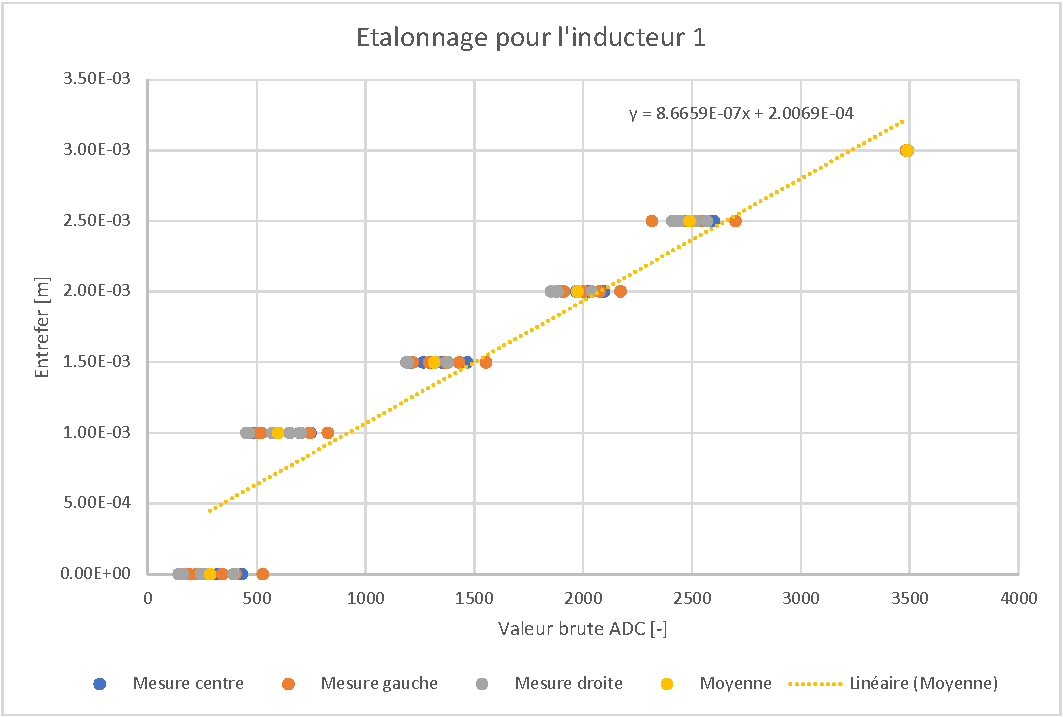
\includegraphics[width=1\linewidth]{assets/content/06-MesureCartePrincipale/EtaADCLin/EtaADCLin-1.pdf}
    \caption{Graphique d'étalonnage de l'ADC de l'inducteur 1 (courbe linéaire)}
    \label{fig:Ind1Lin}
\end{figure}

\begin{figure}[H]
    \centering
    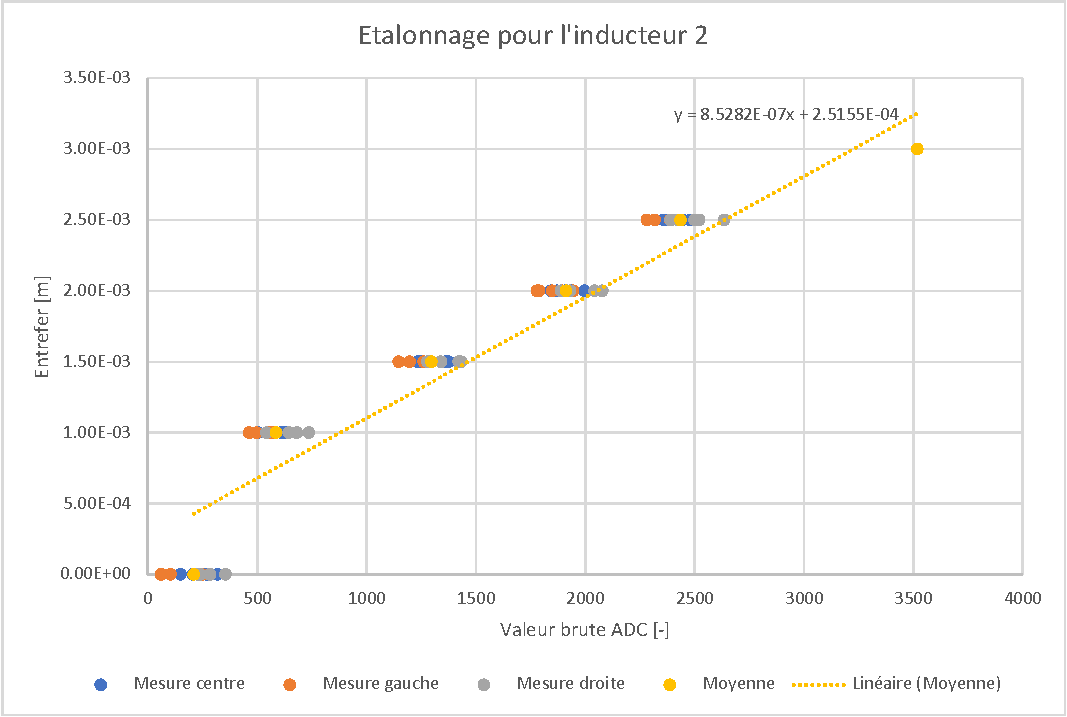
\includegraphics[width=1\linewidth]{assets/content/06-MesureCartePrincipale/EtaADCLin/EtaADCLin-2.pdf}
    \caption{Graphique d'étalonnage de l'ADC de l'inducteur 2 (courbe linéaire)}
    \label{fig:Ind2Lin}
\end{figure}

\begin{figure}[H]
    \centering
    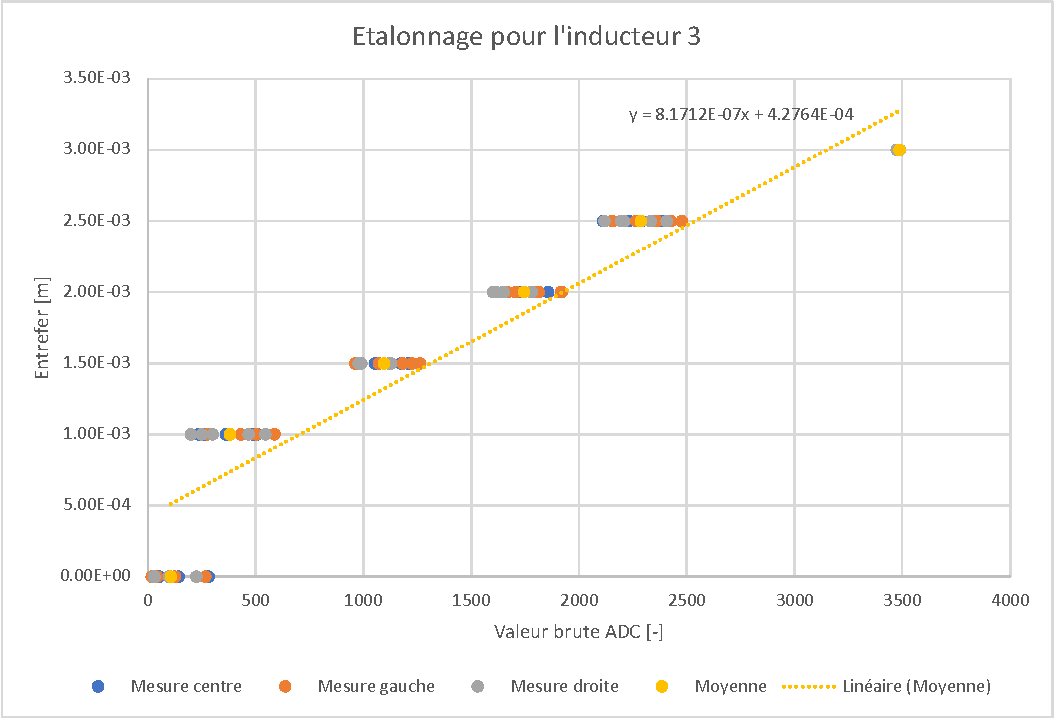
\includegraphics[width=1\linewidth]{assets/content/06-MesureCartePrincipale/EtaADCLin/EtaADCLin-3.pdf}
    \caption{Graphique d'étalonnage de l'ADC de l'inducteur 3 (courbe linéaire)}
    \label{fig:Ind3Lin}
\end{figure}

\begin{figure}[H]
    \centering
    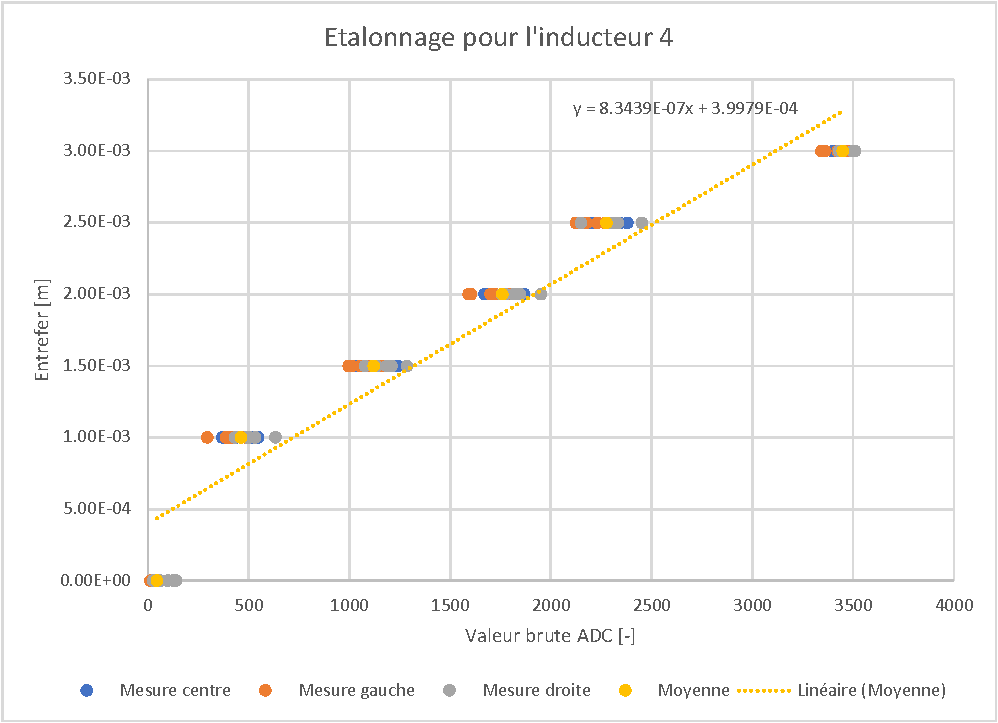
\includegraphics[width=1\linewidth]{assets/content/06-MesureCartePrincipale/EtaADCLin/EtaADCLin-4.pdf}
    \caption{Graphique d'étalonnage de l'ADC de l'inducteur 4 (courbe linéaire)}
    \label{fig:Ind4Lin}
\end{figure}

\subsection{Analyse des résultats}
Le traitement des signaux issus des capteurs de position n'a pas été concluant. Les diverses corrections appliquées présentaient régulièrement de faibles erreurs relatives d'un point de vue théorique, mais ne permettaient jamais d'atteindre un résultat satisfaisant en pratique.

Ces corrections ont été réalisées avant la découverte que la plaque de référence était en réalité ondulée, ce qui a grandement faussé les résultats obtenus.

Il est toutefois intéressant de noter que la calibration « Teach-In » de l'ensemble des capteurs à un niveau de référence commun a semblé améliorer légèrement la stabilité de la maquette. Cette approche nécessite néanmoins de disposer d'une référence fiable.

\section{Conclusion des mesures}
Les premières mesures effectuées sur l'ensemble des convertisseurs ont donné d'excellents résultats, validant ainsi leur bon fonctionnement global.\\

Les relevés liés aux capteurs de courant et à leurs circuits de conditionnement ont montré des écarts par rapport aux valeurs théoriques calculées. Bien que les valeurs obtenues par la méthode inverse, telle qu'implémentée dans le code, diffèrent légèrement des prédictions, la mesure réelle du courant traversant l'inducteur et celle perçue par le capteur restent très proches. Il est donc possible de conclure que le capteur de courant fonctionne correctement.\\

Concernant les mesures de position, bien qu'elles aient régulièrement fourni des données cohérentes, aucune méthode de correction n'a permis d'optimiser efficacement la régulation. La seule intervention ayant montré un effet bénéfique sur la lévitation a été la calibration par la méthode d'apprentissage (« Teach-In ») des capteurs en fixant mécaniquement les inducteurs à un niveau identique.\\

Ces mesures permettent également de statuer sur plusieurs hypothèses de la \autoref{sec:Hypothese} :
\begin{itemize}
    \item L'hypothèse d'une modification de la masse totale est confirmée : la pesée a révélé 18.052~kg au lieu des 13.6~kg considérés jusqu'ici, ce qui fausse les paramètres de la régulation.
    \item L'hypothèse d'un défaut matériel de la carte principale est partiellement confirmée : une broche mal soudée sur le convertisseur 24~V a été détectée et corrigée, mais le reste de l'électronique fonctionne de manière nominale.
    \item L'hypothèse d'une mauvaise calibration globale reste ouverte : aucune correction des capteurs de position n'a suffi à rétablir la lévitation, et la découverte de l'ondulation de la plaque de référence oriente les recherches vers la mesure de cette dernière.
\end{itemize}

En conclusion, l'électronique de la maquette est validée et certifiée fonctionnelle.